\blankpage

%\eachpageornament	
\vspace*{\fill}

\begin{center}
	
\includegraphics[width=\textwidth]{jbw_seal_2000px.png}\\\bigskip
	
	\textit{Published 2020.}
\end{center}

\vspace*{\fill}

\blankpage

%\eachpageornament
\vspace*{\fill}
	
This particular edition of \textit{Eighty Aphorisms and Maxims} was typeset and printed for use by the members of the Martinist Order of Unknown Philosophers, but all seekers of truth are encouraged to find wisdom in these pages.

At the time of publishing, the text of this book is the same as can be found in many places on the Internet, and no attempt has been made to edit or change it other than format it for printing, and to correct transcription errors.

To submit corrections to the text or format, or to ask us a question, please email: 

\url{texanmartinist@gmail.com}

\vspace*{\fill}

\blankpage

\newgeometry{margin=1.2in}

\vspace*{\fill}

	\begin{center}
		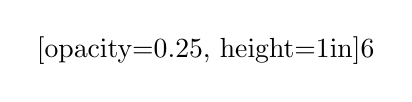
\begin{tikzpicture}
			\node[anchor = north, rotate=0] at (0,0) {\pgfornament[opacity=0.25, height=1in]{6}};
		\end{tikzpicture}
	\end{center}
	
\vspace*{\fill}

\textit{This printing is dedicated to Grand Master Constant Martin Chevillon, \sigi{} (1880 -- 1944), who was martyred in the search of truth, and to all of our Brothers and Sisters in Christ, past, present, and future, who have suffered for their faith.}

\vspace*{\fill}

	\begin{center}
		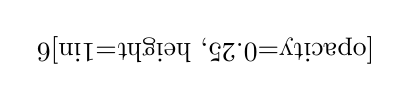
\begin{tikzpicture}
		\node[anchor = north, rotate=180] at (0,0) {\pgfornament[opacity=0.25, height=1in]{6}};
		\end{tikzpicture}
	\end{center}
	
\vspace*{\fill}

\restoregeometry

\blankpage